%% Label Bias and Environmental Datashift
\chapter{Label Bias and Environmental Datashift}
Bias is the result of inadequate data where a certain group or class is favoured over another/others hence creating an overrepresentation \cite{Jiang}\cite{saria2019tutorial}.
ML models trained using such datasets will acquire these underlying biases hence making incorrect predictions.

The following mathematical framework can be used as a representation to undestand bias in data \cite{Jiang}

\begin{figure}[h]
    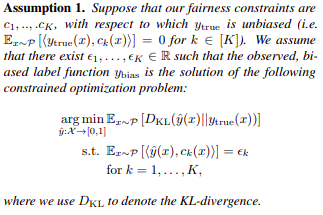
\includegraphics[scale =0.8]{Assumption.png}
    \centering
    \caption{Bias Assumption \cite{Jiang}}
    \label{fig:Assumption}
\end{figure}

In figure \ref{fig:Assumption}, the assumption is that $y_{bias}$ is the label which is closest to $y_{true}$ and achieves the same amount of bias.
In cases where data has been manually manipulated by humans, either consciously or subconsciously, this is deemed to be a reasonable assumption.
The contiguity to $y_{true}$ is given by the KL-divergance, which is used to establish the notion of accurate labeling. 
The Proposition in figure \ref{fig:Proposition} is derived from the KL-divergence. (For complete proof of proposition, see \cite{Jiang})

\begin{figure}[h]
    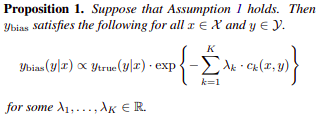
\includegraphics[scale =0.8]{Prop.png}
    \centering
    \caption{Bias Proposition \cite{Jiang}}
    \label{fig:Proposition}
\end{figure}

Now that $y_{bias}$ is represented in terms of $y_{true}$, we can infer $y_{true}$ in terms of $y_{bias}$ as represented in Figure \ref{fig:Corollary}.

\begin{figure}[h]
    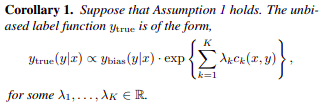
\includegraphics[scale =0.8]{corollary.png}
    \centering
    \caption{Bias Corollary \cite{Jiang}}
    \label{fig:Corollary}
\end{figure}

There may be situations where performance issues may not be apparent during training stages. 
They instead appear post-deployment where training and deployment datasets can have irregularities. 
This is known as Environmental Datashift \cite{saria2019tutorial}. 
This calls into question whether the ML model is robust enough to generalise well to new samples beyond training, or whether it tends to over-generalise to the training dataset thus resulting in unreliability in the real world.


\section{Dataset \& Preprocessing}
The predictive maintenance dataset will be used again to classify failures of an ioT gadget.
During one week, maintenance data was collected from six devices every hour for 168 hrs.
Therefore, this data set contains 1008 rows of data. 
Each cycle of data reading contains the following measurements: 

\section{Results}
\hl{Consider noise in dataset due to uneccassry labels}

Datashift:
\hl{The issue is that modelers typically assume that training data
is representative of the target population or environment where
the model will be deployed} \cite{saria2019tutorial}

\section{Discussion}
